\begin{beamercolorbox}[center,wd=\textwidth]{postercolumn}
        \begin{minipage}[T]{.95\textwidth} % tweaks the width, makes a new \textwidth
          \parbox[t][\columnheight]{\textwidth}{ % must be some better way to set the the height, width and textwidth simultaneously
            % Since all columns are the same length, it is all nice and tidy.  You have to get the height empirically
            % ---------------------------------------------------------%
            % fill each column with content
            
            \begin{block}{4.3 Detecting New Frontiers}
              \begin{itemize}
                \item We scan the calculated contour from previous step
                \item Each point is compared with its (already scanned)
                predecessor
                \item Four possible cases:
                	\begin{itemize}
                	  \item Scanned point is not a frontier point
                	  \item Scanned point is a frontier point but its predecessor is
                	  not
                	  \item Both scanned point and its predecessor are frontier points
                	  \item Scanned point is not a frontier point but its predecessor
                	  is
                	\end{itemize}
                \item Full details can be found in the paper
              \end{itemize}
            \end{block}
            \vfill
            
            \begin{block}{4.4 Maintaining Previously Detected Frontiers}
              \begin{itemize}
              \item \emph{FFD} gains its speed by processing the laser readings
              only
              \begin{itemize}
                \item rather than entire regions of the map
              \end{itemize}
              \item \textbf{Problem}: previously detected frontiers are not
              updated during navigation
              \begin{itemize}
              	\item only the frontier that the robot is headed to
              \end{itemize}
              \item \textbf{Solution}: maintaining frontiers which are not
              covered in the sensors range
              \item \emph{FFD} has to run in the background
               \begin{itemize}
                 \item in contrast to other approaches that are executed in a
                 certain time
               \end{itemize}
              \item \emph{FFD} requires robustness against map orientation
              changes 
	              \begin{itemize}
	                \item caused by loop-closures
	              \end{itemize}
	          \item Avoidance of re-detection of same frontier
	          \item Elimination of previously detected frontiers
	          
              \end{itemize}
              \vskip-0.5ex

              \vskip1ex
              
              \begin{figure}
%                \footnotesize
                %\centering
                \begin{tabular}{p{.35\linewidth}  p{.35\linewidth} }

                  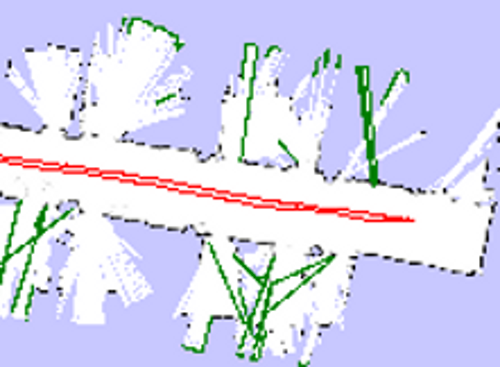
\includegraphics[width=0.6\linewidth]{images/redetecting_bad_example.png}
                  &
                  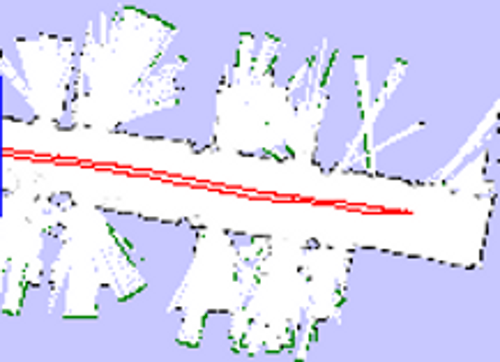
\includegraphics[width=0.6\linewidth]{images/redetecting_good_example.png}
                \end{tabular}
              \end{figure}
            \end{block}
            \vfill
            \begin{block}{5. Experiment Design}
              \begin{itemize}
                \item \emph{WFD} and \emph{FFD} were compared to a
                State of the Art (\emph{SOTA}) algorithm
					\begin{itemize}
					  \item Thanks go to Kai M. Wurm and Wolfram Burgard
					\end{itemize} 
                \item Our system is based on \emph{GMapping} SLAM implementation
                \newline [Grisetti, Stachniss and Burgard (2007)]
                \item We used several environments taken from RADISH
                [Howard and Roy (2003)]
                \item We use raw sensor readings and odometry:
                	\begin{itemize}
                	  \item All algorithms use exactly the same data
                	  \item All algorithms form the same robot trajectories
                	  \item The movement of the robot is identical
                	  \item The only thing we examine is how quickly it can compute
                	  frontiers
                	\end{itemize} 
              \end{itemize}
              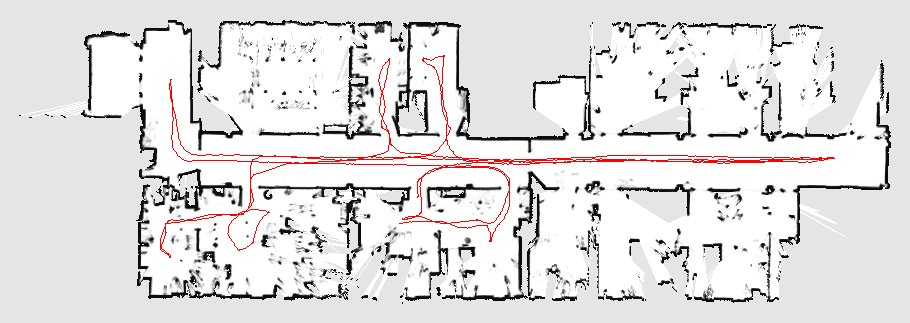
\includegraphics[width=0.5\linewidth]{images/freiburg.JPG}
              
            \end{block}
            \vfill
            
            \begin{block}{6. Results: SOTA vs. WFD vs. FFD}
             \begin{columns}
                \begin{column}{.5\textwidth}
                  \begin{itemize}
		              \item Intel Core 2 Duo T6600 CPU
		              \item Clock speed of 2.20 GHz
		              \item RAM in size of 4GB
		              
	              \end{itemize}
 	             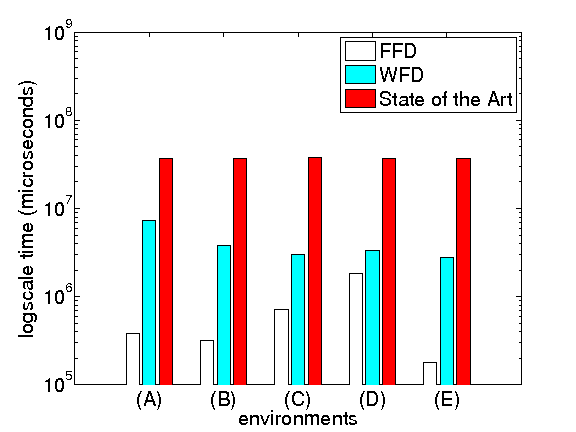
\includegraphics[width=0.7\linewidth]{images/graph_Results_core2.png}
 	             \vskip-0.5ex
                \end{column}
                \begin{column}{.5\textwidth}                
          %        \vskip-3ex
                     \begin{itemize}
		              \item Intel Pentium III (Coppermine) CPU
		              \item Clock speed of 800 MHz
		              \item RAM in size of 1GB
		              
	              \end{itemize}
	 	              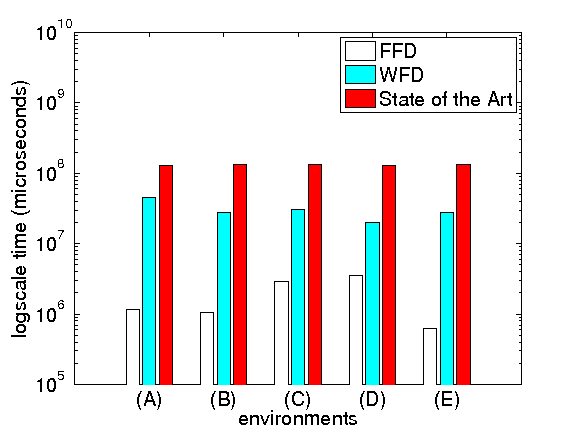
\includegraphics[width=0.7\linewidth]{images/graph_Results_coppermine.png}
	 	              \vskip-0.5ex
                \end{column}
              \end{columns} 
			 
              \vskip-0.5ex

            \end{block}
            \vfill
            \begin{block}{7. Conclusions and Future Work}
              \begin{itemize}
              \item Reducing frontier detection time can reduce exploration time
              \item We introduced two novel faster frontier detectors
              \item \emph{FFD} outperforms \emph{WFD} and \emph{SOTA}
              by 1-2 orders of magnitude
			  \item Future: investigate exploration policies, based on
			  real-time frontier detection
              \end{itemize}
            \end{block}
          }
          % ---------------------------------------------------------%
          % end the column
        \end{minipage}
      \end{beamercolorbox}
